\section{Process View}
De process view van het 4 + 1 model dient om het run-time gedrag van het systeem in beeld te brengen \parencite{4+1ViewModelPaper}.
In deze sectie wordt er gekeken hoe het ophalen van de data vanuit de backend werkt.
Verder wordt er ook gekeken hoe de data gerenderd wordt in de frontend.

\subsection{Backend}
Om het proces van het ophalen van de data in beeld te krijgen is er gebruik gemaakt van een sequencediagram.
In figuur \ref{fig:SequenceDiagramItemValueWithChildren} is te zien dat er 4 lagen zijn. 
Dit zijn de Controller, Datahandler, handler en access layer.
De logica om te bepalen of het een succesvolle request was zit in de datahandler.
Logica om het verwachte object terug te krijgen zit in de handler.
En als laatste is er de access layer die de data uit de database haalt.

\whitespace
\begin{graphic}
    \captionsetup{type=figure}
    \caption{Sequencediagram ItemValue}
    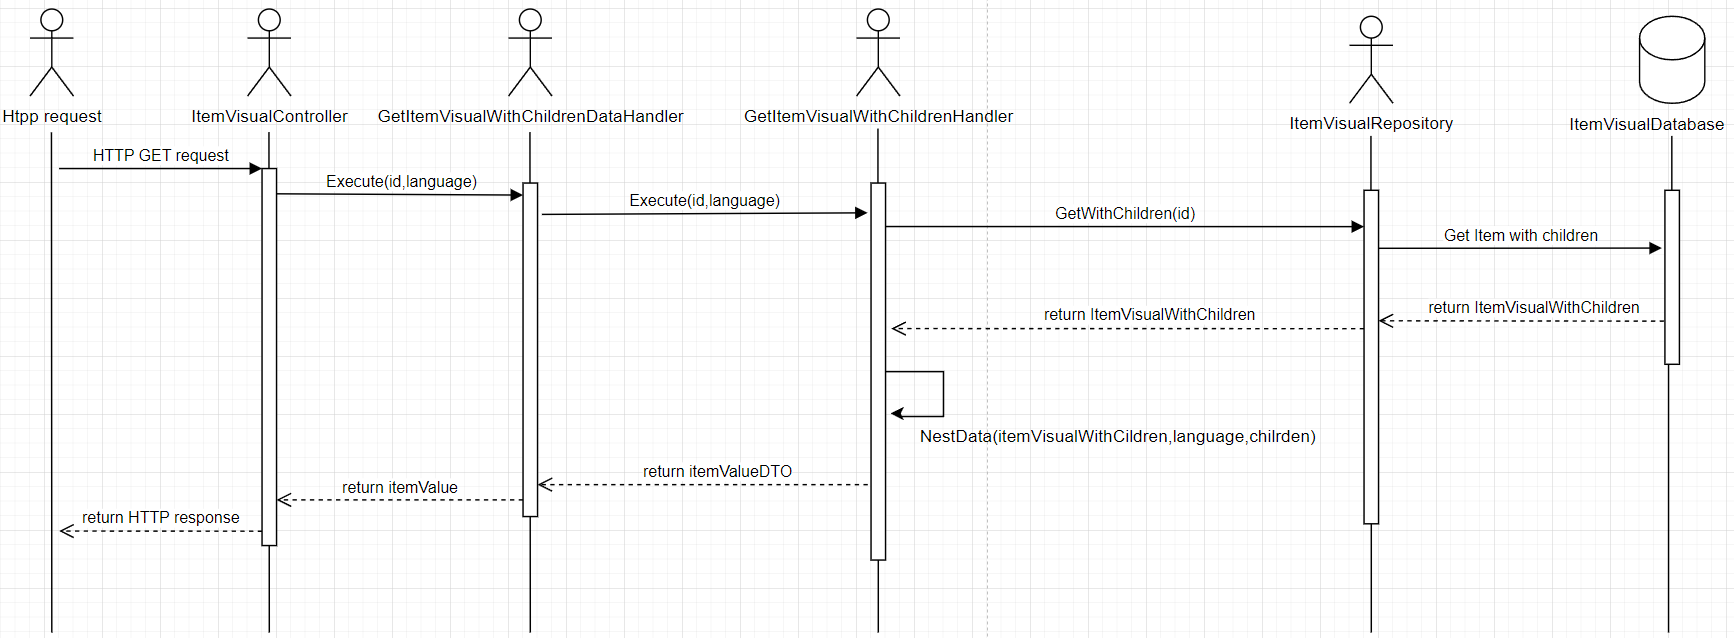
\includegraphics[scale=0.4]{SequenceDiagramItemValueWithChildren.png}
    \label{fig:SequenceDiagramItemValueWithChildren}
\end{graphic}

% \whitespace
% Een belangrijke functionaliteit in het nesten van de data zodat de frontend het makkelijk kan renderen.
% Dit wordt gedaan in de NestData functie om meer inzicht te geven van het proces van de functie is er een flowchart gemaakt (zie figuur \ref{fig:FlowchartNestData}).
%
% \whitespace[2]
% \begin{graphic}
%     \captionsetup{type=figure}
%     \caption{flowchart diagram NestData}
%     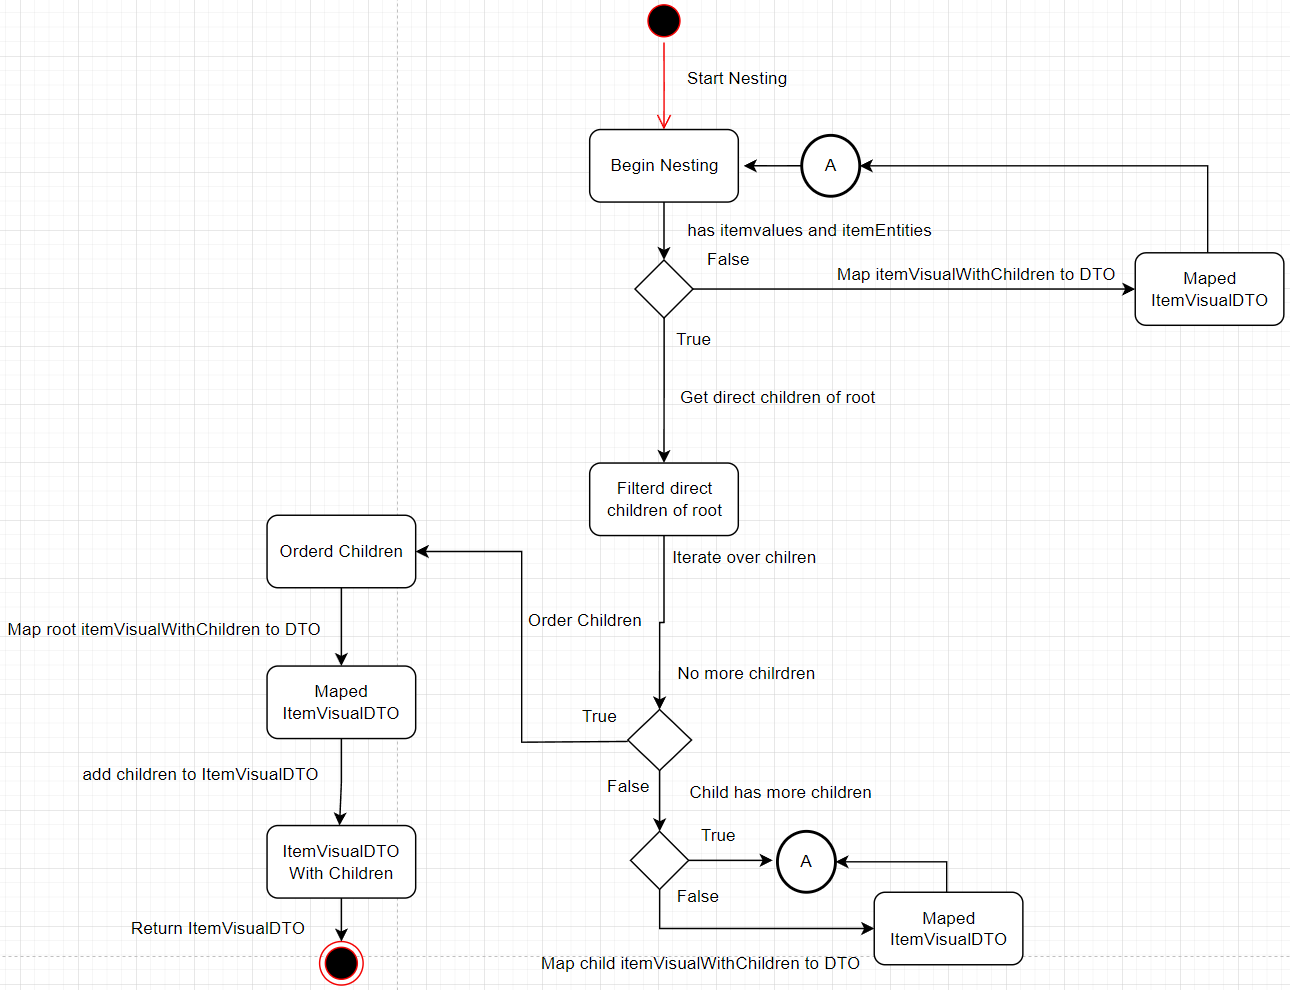
\includegraphics[scale=0.3]{NestingDataFlowchart.png}
%     \label{fig:FlowchartNestData}
% \end{graphic}

\newpage
\subsection{Frontend}

Om de data te renderen wordt er gebruikgemaakt van 2 verschillende entiteiten types.
Type 1 is een voor gedefinieerd component, hier bij kun je denken aan een artikel, card, afbeelding etc.
Het andere type is een generiek component dat het type 1 componenten encapsuleerd.
Deze componenten worden containers genoemd omdat ze verschillende items encapsuleren.
Verder kunnen containers ook meerdere containers encapsuleren.

\whitespace
\begin{graphic}
    \captionsetup{type=figure}
    \caption{flowchart diagram frontend}
    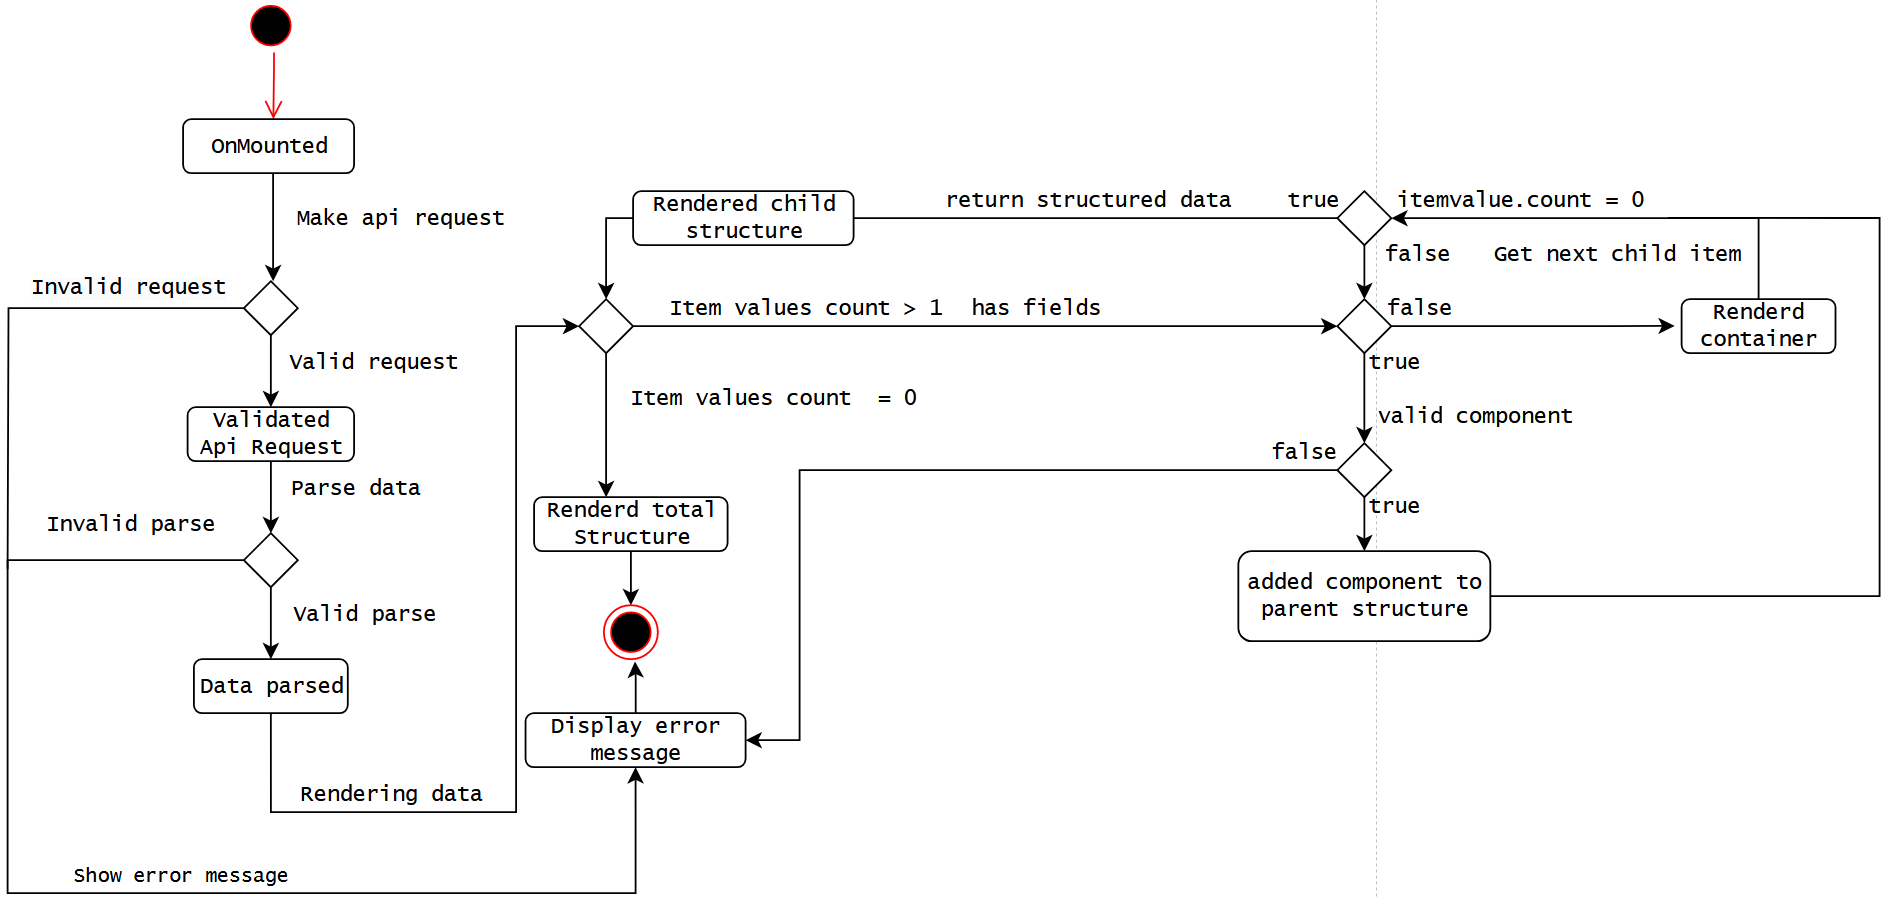
\includegraphics[scale=0.34]{FlowchartFrontend.png}
    \label{fig:FlowchartFrontend}
\end{graphic}

\whitespace
In figuur \ref{fig:FlowchartFrontend} wordt er getoond hoe de frontend met deze container structuur om gaat.
Na het initiële ophalen en valideren van de data begint de main loop van de frontend.
Eerst wordt er gekeken of het huidige object 1 of meer items heeft.
Daarna wordt elk item gerenderd en als het een container is, wordt deze recursief ook gerenderd.
Dit gaat door tot dat alle items gerenderd zijn.

